\documentclass[tikz,border=3.14pt]{standalone}
\usepackage{xcolor}
\usetikzlibrary{3d,decorations.text,shapes.arrows,positioning,fit,backgrounds}
\usetikzlibrary{shapes.geometric, arrows.meta}
\usetikzlibrary{arrows.meta, positioning}
\tikzset{
    pics/fake box/.style args={#1 with dimensions #2 and #3 and #4}{
        code={
            \draw[gray,ultra thin,fill=#1] (0,0,0) coordinate(-front-bottom-left) --++
                (0,#3,0) --++
                (#2,0,0) --++
                (0,-#3,0) -- cycle;
            \draw[gray,ultra thin,fill=#1] (0,#3,0) --++
                (0,0,#4) --++
                (#2,0,0) --++
                (0,0,-#4) -- cycle;
            \draw[gray,ultra thin,fill=#1!80!black] (#2,0,0) --++
                (0,0,#4) --++
                (0,#3,0) --++
                (0,0,-#4) -- cycle;
        }
    },
    circle dotted/.style={dash pattern=on .05mm off 2mm,line cap=round}
}

\definecolor{yell1}{RGB}{254,246,184}
\definecolor{blu1}{RGB}{149,208,251}
\definecolor{red1}{RGB}{246,182,171}
\definecolor{gren1}{RGB}{169,213,152}

\tikzstyle{block} = [rectangle, draw=black, fill=yell1, 
    minimum width=3cm, minimum height=3cm, text width=0.75cm, text centered]

\tikzstyle{se} = [rectangle, draw=black, fill=blu1, 
    minimum width=3cm, minimum height=0.75cm, text width=3cm, text centered]

\tikzstyle{se2} = [rectangle, draw=black, fill=gray!20, 
    minimum width=2cm, minimum height=0.75cm, text width=2cm, text centered]

\tikzstyle{gap} = [rectangle, draw=black, fill=red1, 
    minimum width=3cm, minimum height=0.75cm, text width=3cm, text centered]

\tikzstyle{fc} = [rectangle, draw=black, fill=gren1, 
    minimum width=3cm, minimum height=0.75cm, text width=3cm, text centered]

\tikzstyle{startend} = [rectangle, draw=black, fill=white, 
    minimum width=3cm, minimum height=0.75cm, text width=3cm, text centered]

\tikzstyle{arrow} = [thick,->,>=stealth]

\begin{document}



% \begin{tikzpicture}[x={(1,0)},y={(0,1)},z={({cos(60)},{sin(60)})},
%     font=\sffamily\small,scale=2]

% % ========= Convolutional Blocks =========
% % image input
% % \pic at (-1.5,0,0) {fake box=white!70!gray with dimensions 0 and 12 and 10};

% % % == CONV1 ==%
% % \pic at (0, 0,0) {fake box=white!70!green with dimensions 0.25 and 12 and 10};
% % \pic at (0.125, 1.5, 1.5) {fake box=white!70!cyan with dimensions 0.25 and 6 and 4};
% % % \draw[-latex,thick] (0.25, 3, 2.5) --++ (0.75, 0, 0);
% % % \node[above] at (0.4, 2.1, 0) {Block 1};

% % % == CONV2 ==%
% % \pic at (0.5, 1.5, 1.5) {fake box=white!70!green with dimensions 0.5 and 6 and 4};
% % \pic at (0.75, 2.25, 2) {fake box=white!70!cyan with dimensions 0.5 and 3 and 2};
% % % \draw[-latex,thick] (2, 3, 2.5) --++ (0.5, 0, 0);

% % % == CONV3 ==%
% % \pic at (1.25, 2.25, 2) {fake box=white!70!green with dimensions 1.0 and 3 and 2};
% % \pic at (1.75, 2.625, 2.25) {fake box=white!70!cyan with dimensions 1.0 and 1.5 and 1.0};
% % % \draw[-latex,thick] (3.75, 3, 2.5) --++ (0.625, 0, 0);

% % % == CONV4 ==%
% % \pic at (2.5, 2.625, 2.25) {fake box=white!70!green with dimensions 2.0 and 1.5 and 1.0};
% % \pic at (3.5, 2.8125, 2.375) {fake box=white!70!cyan with dimensions 2.0 and 0.75 and 0.5};
% % % \draw[-latex,thick] (6.5, 3, 2.5) --++ (0.75, 0, 0);

% % % == CONV5 ==%
% % \pic at (4.75, 2.8125, 2.375) {fake box=white!70!green with dimensions 4.0 and 0.75 and 0.5};
% % \pic at (6.75, 2.90625, 2.4375) {fake box=white!70!cyan with dimensions 4.0 and 0.375 and 0.25};

% % \pic at (1.5,0,0) {fake box=white!70!gray with dimensions 0.8 and 1.6 and 1.2};
% % % \node[above] at (1.9, 1.7, 0) {Block 2};

% % \draw[-latex,thick] (2.3,0.8,0.5) --++ (0.7,0,0);

% % \pic at (3.0,0,0) {fake box=white!70!gray with dimensions 0.8 and 1.2 and 1.0};
% % \node[above] at (3.4, 1.3, 0) {Block 3};

% % \draw[-latex,thick] (3.8,0.6,0.5) --++ (0.7,0,0);

% % \pic at (4.5,0,0) {fake box=white!70!gray with dimensions 0.8 and 1.0 and 0.8};
% % \node[above] at (4.9, 1.1, 0) {Block 4};

% % \draw[-latex,thick] (5.3,0.5,0.5) --++ (0.7,0,0);

% % \pic at (6.0,0,0) {fake box=white!70!gray with dimensions 0.8 and 0.8 and 0.6};
% % \node[above] at (6.4, 0.9, 0) {Block 5};

% % \draw[-latex,thick] (6.8,0.4,0.5) --++ (0.7,0,0);

% % ========= SE Block =========
% % \node[draw, single arrow, orange, fill=orange!30, minimum height=0.8cm, minimum width=1cm] (SE) at (8,0,0) {SE};

% % \draw[-latex,thick] (7.5,0.5,0.5) -- (SE.west);

% % ========= GAP =========
% % \node[draw, single arrow, orange, fill=orange!50, minimum height=0.8cm, minimum width=1.2cm] (GAP) at (9.2,0,0) {GAP};

% % \draw[-latex,thick] (SE.east) -- (GAP.west);

% % ========= Fully Connected Layers =========
% % \node[circle,draw,blue,fill=blue!30,minimum size=0.5cm,right=1.2cm of GAP] (FC1) {};
% % \node[circle,draw,red,fill=red!30,below=0.6cm of FC1] (FC2) {};
% % \node[circle,draw,green,fill=green!30,below=0.6cm of FC2] (FC3) {};
% % \draw[circle dotted, line width=2pt,shorten <=3pt] (FC2) -- (FC3);

% % \draw[-latex,thick] (GAP.east) -- (FC1.west);

% % ========= Dense Output =========
% % \node[circle,draw,gray,fill=gray!20,right=1.2cm of FC1] (D1) {};
% % \node[circle,draw,gray,fill=gray!60,below=0.6cm of D1] (D2) {};
% % \node[circle,draw,gray,fill=gray!20,below=0.6cm of D2] (D3) {};
% % \draw[circle dotted, line width=2pt,shorten <=3pt] (D2) -- (D3);

% % \foreach \X in {FC1, FC2, FC3}
% % {
% %     \draw[-latex,thick] (\X) -- (D2.west);
% % }

% % ========= Background highlighting =========
% % \begin{scope}[on background layer]
% %     \node[orange!20,rounded corners,fit=(FC1) (FC3),inner sep=8pt]{};
% %     \node[gray!10,rounded corners,fit=(D1) (D3),inner sep=8pt]{};
% % \end{scope}



% \end{tikzpicture}

% CNN
% \begin{tikzpicture}[node distance=0cm and 0.5cm]
%     % Rotated text manually inside each node using \rotatebox
%     \node (image) [startend] {\rotatebox{90}{Wafer Image}};
%     \node (cb1) [block, right=of image] {\rotatebox{90}{ConvBlock1}};
%     \node (cb2) [block, right=of cb1] {\rotatebox{90}{ConvBlock2}};
%     \node (cb3) [block, right=of cb2] {\rotatebox{90}{ConvBlock3}};
%     \node (cb4) [block, right=of cb3] {\rotatebox{90}{ConvBlock4}};
%     \node (cb5) [block, right=of cb4] {\rotatebox{90}{ConvBlock5}};
%     \node (se) [se, right=of cb5] {\rotatebox{90}{SE Block}};
%     \node (gap) [gap, right=of se] {\rotatebox{90}{GAP Block}};
%     \node (fc1) [fc, right=of gap] {\rotatebox{90}{FC 1}};
%     \node (fc2) [fc, right=of fc1] {\rotatebox{90}{FC 2}};
%     \node (out) [startend, right=of fc2] {\rotatebox{90}{Defect Class}};
    
%     \node[below=0.2cm of image] {\tiny $[1,256,256]$};
%     \node[below=0.2cm of cb1] {\tiny $[32,128,128]$};
%     \node[below=0.2cm of cb2] {\tiny $[64,64,64]$};
%     \node[below=0.2cm of cb3] {\tiny $[128,32,32]$};
%     \node[below=0.2cm of cb4] {\tiny $[256,16,16]$};
%     \node[below=0.2cm of cb5] {\tiny $[512,8,8]$};
%     \node[below=0.2cm of se] {\tiny $[512,8,8]$};
%     \node[below=0.2cm of gap] {\tiny $[512]$};
%     \node[below=0.2cm of fc1] {\tiny $[512]$};
%     \node[below=0.2cm of fc2] {\tiny $[128]$};
%     \node[below=0.2cm of out] {\tiny $[8]$};

%     % Arrows
%     \draw [arrow] (image) -- (cb1);
%     \draw [arrow] (cb1) -- (cb2);
%     \draw [arrow] (cb2) -- (cb3);
%     \draw [arrow] (cb3) -- (cb4);
%     \draw [arrow] (cb4) -- (cb5);
%     \draw [arrow] (cb5) -- (se);
%     \draw [arrow] (se) -- (gap);
%     \draw [arrow] (gap) -- (fc1);
%     \draw [arrow] (fc1) -- (fc2);
%     \draw [arrow] (fc2) -- (out);
%     % \draw [arrow] (relu) -- (pool);
% \end{tikzpicture}

% \begin{tikzpicture}[node distance=0.5cm]
%     % Rotated text manually inside each node using \rotatebox
%     \node (image) [startend] {Wafer Image};
%     \node (reshape) [se, below=of image] {Reshape};
%     \node (centers) [se2, left=of reshape] {Centers};
%     \node (distance) [se, below=of reshape, yshift=-0.75cm] {Distance};
%     \node (rbf) [se, below=of distance] {RBF Kernel ($\phi$)};
%     \node (fc) [fc, below=of rbf] {FC};
%     \node (out) [startend, below=of fc] {Defect Class};

%     \node[draw,
%         circle,
%         minimum size=0.6cm,
%         fill=blu1
%     ] (sum) at (0,-2.25){};

%     \draw (sum.north east) -- (sum.south west)
%         (sum.north west) -- (sum.south east);
%     \node[left=-1pt] at (sum.center){\tiny $-$};
%     \node[above] at (sum.center){\tiny $+$};
    
%     % \node[below=0.2cm of image] {\tiny $[1,256,256]$};

%     % Arrows
%     \draw [arrow] (image) -- (reshape);
%     \draw [arrow] (distance) -- (rbf);
%     \draw [arrow] (rbf) -- (fc);
%     \draw [arrow] (fc) -- (out);
%     \draw [arrow] (reshape) -- (sum.north);
%     \draw [arrow] (sum.south) -- (distance);
%     \draw [arrow] (centers) |- (sum.west);
% \end{tikzpicture}

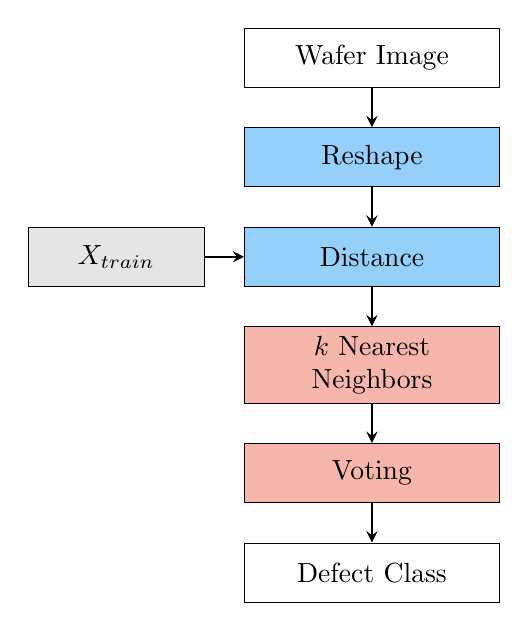
\begin{tikzpicture}[node distance=0.5cm]
    % Rotated text manually inside each node using \rotatebox
    \node (image) [startend] {Wafer Image};
    \node (reshape) [se, below=of image] {Reshape};
    \node (dist) [se, below=of reshape] {Distance};
    \node (train) [se2, left=of dist] {$X_{train}$};
    \node (knn) [gap, below=of dist] {$k$ Nearest Neighbors};
    \node (vote) [gap, below=of knn] {Voting};
    \node (out) [startend, below=of vote] {Defect Class};

    % Arrows
    \draw [arrow] (image) -- (reshape);
    \draw [arrow] (reshape) -- (dist);
    \draw [arrow] (dist) -- (knn);
    \draw [arrow] (knn) -- (vote);
    \draw [arrow] (vote) -- (out);
    \draw [arrow] (train) -- (dist);
\end{tikzpicture}
\end{document}